\documentclass{article}
\usepackage{listings}
\usepackage[numbers]{natbib}
\usepackage[only,llbracket,rrbracket,llparenthesis,rrparenthesis]{stmaryrd}
\usepackage{graphicx}
\usepackage{graphicx,sidecap,tikz}
\usepackage{fontspec}
\usepackage{hyphenat}
\usepackage[english,russian]{babel}
\usepackage{amsmath}
\usepackage{amssymb}
\usepackage{txfonts}
\usepackage[utf8]{inputenc}
\usepackage{url}

\newcommand*{\thead}[1]{\multicolumn{1}{c}{\bfseries #1}}

\fontencoding{T1}
\newfontfamily{\cyrillicfont}{Geometria}
\setmainfont{Geometria}

\addto\captionsrussian{\renewcommand{\contentsname}{Зміст}}
\addto\captionsrussian{\renewcommand{\bibname}{Бібліографія}}
\addto\captionsrussian{\renewcommand{\abstractname}{Анотація}}

\begin{document}

\title{Коцептуальна модель системи доведення теорем}
\author{Maksym Sokhatskyi $^1$ and Pavlo Maslianko $^1$}
\date{
    $^1$ National Technical University of Ukraine \\
    \small Igor Sikorsky Kyiv Polytechnical Institute\\
    \small 18 травна 2018 року
}

\maketitle

\begin{abstract}
Дана робота презентує концептуальну модель системи доведення теорем, яка предствалена як система:
1) числень разом з їх категорними моделями [статика], тобто властивостями та семантикою;
2) програм та базових бібліотек [екземпляри], для програмного забезпечення;
3) програмних трансформацій між різними численнями [динаміка], компіляція, екстракт програм в інші мови програмування, оптимізація, тощо.
Значна увага приділена таким проблемам як: 1) масштабування системи доведення теорем
на довільні числення; 2) декомпозиції системи мовні рівні.
В основу роботи покладені сучасні фундаментальні дослідження з кубічної теорії типів,
що дозволяє формулювати і доводити гомотопічні моделі та їх властивості.
\end{abstract}

\newpage
\tableofcontents
\newpage

\section{Вступ}

\subsection{Актуальність роботи}
Ціна помилок в індустрії надзвичайно велика. Наведемо
відомі приклади: 1) Mars Climate Orbiter (1998), помилка невідповідності
типів британської метричної системи, коштувала 80 мільйонів фунтів стерлінгів.
Невдача стала причиною переходу NASA повністю на метричну систему в 2007 році.
2) Ariane Rocket (1996), причинан катастрофи -- округлення 64-бітного дійсного
числа до 16-бітного. Втрачені кошти на побудову ракети та запуск 500 мільйонів
3) Помилка в FPU в перших Pentium (1994), збитки на 300 мільйонів.
4) Помилка в SSL (heartbleed), оцінені збитки у розмірі 400 мільйонів.
5) Помилка у логіці бізнес-контрактів EVM та
DAO (неконтрольована рекурсія), збитки 50 мільйонів.
Більше того, і найголовніше, помилки у програмному забезпеченні можуть
коштувати життя людей.

\subsection{Верифікація та валідація}
Для унеможливлення помилок на виробництві застосовуються різні
методи формальної верифікації. Формальна верифікація — доказ, або заперечення
відповідності системи у відношенні до певної формальної специфікації або характеристики,
із використанням формальних методів математики.

Дамо основні визначення згідно з міжнародними нормами (IEEE, ANSI)\footnote{IEEE Std 1012-2016  --- V\&V Software verification and validation} та у відповідності до вимог
Європейського Аерокосмічного Агенства\footnote{ESA PSS-05-10 1-1 1995 -- Guide to software verification and validation}.
У відповідності до промислового процессу розробки, верифікація та валідація програмного
забезпечення є частиною цього процесу. Програмне забезпечення перевіряється на
відповідність функціональних властивостей згідно вимог.

Процес валідації включає в себе перегляд (code review),
тестування (модульне, інтеграційне, властивостей), перевірка моделей, аудит,
увесь комплекс необхідний для доведення, що продукт відповідає вимогам
висунутим при розробці. Такі вимоги формуються на початковому етапі,
результатом якого є формальна специфікація.

\subsection{Формальна специфікація}
Для спрощення процесу верифікації та валідації
застосовується математична техніка формалізації постановки задачі --- формальна специфікація.
Формальна специфікація --- це математична модель, створена для опису систем,
визначення їх основних властивостей, та інструментарій для перевірки
властивостй (формальної верифікаціїї) цих систем, побудованих на основі формальної специфікації.

Існують два фундаментальні підходи до формальних специфікацій: 1) Аглебраїчний підхід, де
система описується в термінах операцій, та відношень між ними, та
2) Модельно-орієнотований підхід, де модель створена конструктивними побудовами,
як то на базі теорії множин, чи інкаше, а системні операції визначаються тим, як вони змінюють
стан системи. Також були створені сімейства послідованих та розподілених мов.

Найбільш стандартизована та прийнята в обсласті формальної верификації --- це нотація
Z\footnote{ISO/IEC 13568:2002 --- Z formal specification notation} (Spivey, 1992), приклад
модельно-орієнтовоної мови
Назавана у честь Ернеста Цермело, роботи якого мали вплив на фундамент математики та аксіоматику
теорії множин. Саме теорія множин, та логіка предикатів першого порядку є теорією мови Z.

Інша відома мова формальної специфікації як стандарт для моделювання розподілених систем,
таких як телефонні мережі та протоколи, це
LOTOS\footnote{ISO 8807:1989 --- LOTOS --- A formal description technique based
on the temporal ordering of observational behaviour} (Bolognesi, Brinksma, 1987), як приклад алгебраїчного підходу.
Ця мова побудована на темпоральних логіках, та поведінках залежниих від спостережень.
Інші темпоральні мови специфікацій, які можна відзначити тут --- це TLA+\footnote{The
TLA+ Language and Tools for Hardware and Software Engineers}, CSP (Hoare, 1985),
CCS\footnote{J.C.M. Baeten. A Brief History of Process Algebra.} (Milner, 1971), Actor Model, Reactive Streams, etc.

\section{Формальні методи верифікації}


\subsection{Історія систем доведення теорем}
Перші спроби пошуку формального фундаменту для теорії обчислень були покладені
Алонзо Черчем та Хаскелем Каррі у 30-х роках 20-го століття. Було запропоноване
лямбда числення як апарат який може замінити класичну теорію множин та її аксіоматику,
пропонуючи при цьому обчислювальну семантику. Пізніше в 1958, ця мова була втілена
у вигляді LISP лауреатом премії тюрінга Джоном МакКарті, який працював в Прінстоні.
Ця мова була побудована на конструктивних примітивах, які пізніше виявилися компонентами
індуктивних конструкцій та були формалізовані за допомогою
теорії категорій Вільяма Лавіра. Окрім LISP, нетипізоване лямбда числення
маніфестується у такі мови як Erlang, JavaScript, Python.
До цих пір нетипізоване лямбла числення є одною з мов у які робиться
конвертація доведених программ (екстракція).

Перший математичний прувер AUTOMATH (і його модифікації AUT-68 та AUT-QE),
який був написаний для комп'ютерів розроблявся під керівництвом де Брейна, 1967.
У цьому прувері був квантор загальності та лямбда функція, таким чином це був перший прувер
побудрваний на засадах ізоморфізма Каррі-Говарда-Ламбека.

ML/LCF або метамова і логіка обчислювальних функцій були наступним кроком до
осягнення фундаментальної мови простору, тут вперше з'явилися алебраїчні типи даних
у вигляді індуктивних типів, поліноміальних функторів або термінованих (well-founded) дерев.
Роберт Мілнер, асистований Морісом та Н'юві розробив Метамову (ML), як
інструмент для побудови прувера LCF. LCF був основоположником у родині пруверів
HOL88, HOL90, HOL98 та останньої версії на даний час HOL/Isabell.
Пізніше були побувані категорні моделі Татсоя Хагіно (CPL, Японія)
та Робіна Кокета (Charity, Канада).

У 80-90 роках були створені інші системи автоматичного доведення теорем,
такі як Mizar (Трибулєк, 1989). PVS (Оур, Рушбі, Шанкар, 1995),
ACL2 на базі Common Lisp (Боєр, Кауфман, Мур, 1996), Otter (МакКюн, 1996).

\subsection{Системи моделювання та верифікації}
Можна виділити три підходи до верифікації.
Перший застосовується де вже є
певна програма написана на певній мові програмування і потрібно довести ізоморфність
цієї програми до доведеної моделі. Ця задача вирішується у побудові теоретичної моделі
для певної мови програмування, потім програма на цій мові переводиться у цю
теоретичну модель і доводить ізоморфізм цієї програми у побудованій моделі до доведеної моделі.
Приклади таких систем та піходів: 1) VST (CompCert, сертифікація C програм),
2) NuPRL (Cornell University, розподілені системи, залежні типи),
3) TLA+ (Microsoft Reseach, Леслі Лампорт),
4) Twelf (для верифікації мов програмування), 5) SystemVerilog (для
ч'програмного та апаратного забезпечення).

\subsection{Мови з залежними типами}
Другий підхід можна назвати підходом вбудованих мов.
Компілятор основої мови перевіряє модель закодовану у ній же. Можливо моделювання
логік вищого порядку, лінійних логік, модальних логік, категорний та гомотопічних логік.
Процес специфікації та верифікації відбувається в основній мові, а сертифіковані програми
автоматично екстрагуються в довільні мови.
Приклади таких систем: 1) Coq побудована на мові OCaml від науково-дослідного
інституту Франції INRIA; 2) Agda побудовані на мові Haskell від шведського інституту технологій Чалмерс;
3) Lean побудована на мові C++ від Microsoft Research та Універсистету Каргені-Мелона;
4) Idris подудована на мові Haskell Едвіна Бреді з шотландського Університету ім. св. Андрія;
5) F* -- окремий проект Microsoft Research.

\subsection{Системи автоматичного доведення теорем}
Третій підхід полягає в синтезі конструктивного доведення
для формальної специфікації. Це може бути зроблено за
допомогою асистентів доведення теорем, таких як HOL/Isabell, Coq, ACL2,
або систем розв'язку задач виконуваності формул в теоріях (Satisfiability Modulo Theories, SMT).

\subsection{Обмеження}
Незалежно від піходу до верифіції, формальна верифікація неможлива,
якщо мова програмування моделі формально не визначена. Це означає шо значна міра
програмного забезпечення може бути автоматично верифікована тільки для тих мов,
формальні моделі яких побудовані, на даний момент це тільки мова С.
Більше того, не завжди можна також формально довести те, що програма завершиться,
потрібно звужувати клас програм, якщо формальні специфікації містять такі властивості.

\section{Формалізована постановка задачі}

\subsection{Об'єкт дослідження}
Об'єктом дослідження данної роботи є:
1) системи верифікації програмного забезпечення;
2) системи доведення теорем;
3) мови програмування;
4) операційні системи, які виконують обчислення в реальному часі;
3) їх поєднання, побудова формальної системи для
унифікованого середовища, яке поєднує середовище виконання та систему
верифікації у єдину систему мов та засобів.

\subsection{Предмет дослідження}
Предметом дослідження такої системи мов є теорія типів, яка вивчає обчислювальні властивості мов.
Теорія типів виділилася в окрему науку завдяки роботам Бішопа та Мартіна-Льофа, як запит на вакантне місце у
трикутнику теорій, які відповідають ізоморфізму Каррі-Говарда-Ламбека (Логіки, Мови, Категорії),
або інтерпретації Брауера-Гейтінга-Колмогорова. Інші дві це: теорія категорій та логіки вищих порядків.

\subsection{Мотивація}
Одна з причина низького рівня впровадження у виробництво систем
верифікації -- це висока складність таких систем. Складні системи
верифікуються складно. Ми хочемо запропонувати спрощений
підхід до верифікації -- оснований на концепції компактних
та простих мовних ядер для створення специфікацій, моделей,
перевірки моделей, доведення теорем у теорії типів з кванторами.

\subsection{Завдання дослідження}
Завдання дослідження полягає у:
1) декомпозіції типових систем,
побудові єдиної категорії мов программуваня, де
об'єкти --- це мови програмування, а морфізми --- це мовні перетворення;
2) виділенні мінімальної конфігурації яка дозволяю доводити
властивості програмного забезпечання на усіх етапах від проектування до виконання;
3) побудові гнучкої поліморфної системи мовних розширень до
мінімального ядра для забезпечення потреб масшабування системи;
4) реалізації мінімального ядра системи та вищих мовних
розширень разом із базовими бібліотеками.

\subsection{Структура дослідження}
Структура дослідження відображає компонентну модель системи доведення теорем:
1) інтерпретатор безтипового лямбда числення;
2) компактне ядро --- система з однією аксіомою;
3) мова з індуктивними типами;
4) мова з гомотопічним інтервалом $[0,1]$;
5) уніфікована базова бібліотека.

\section{Мінімальна верифікована система програмування}

Пошук мінімальної конфугурації мов визначається мотивацією дослідження,
як запорука прозорості та адаптованості до безкоштовної верифікації
або верифікації малими зусиллями.

\begin{figure}[h]
  \centerline{\includegraphics[scale=0.28]{minimal}}
  \caption{The Stages of Model Verifications}
\end{figure}

\subsection{Інтерпретатор безтипового лямбда числення}

Чому саме інтерпретатор?
Як можна побудувати ефективний інтерпретатор?
Нормальний та зворотній порядок бета редукції.
Векторизація обчислень.

\subsection{Чиста система з однією аксіомою}

Чиста система.
Операційна семантика.
Категорна семантика залежної теорії.

\section{Вищі мови програмування}

Математична індукція.
Топологічні та гомотопічні моделі.

\begin{figure}[h]
  \centerline{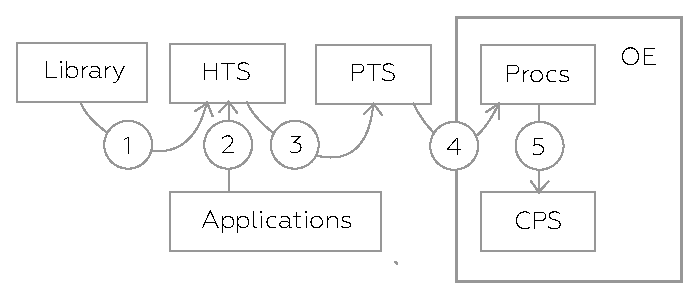
\includegraphics[scale=0.28]{higher}}
  \caption{The Stages of Model Verifications}
\end{figure}

\subsection{Індуктивні мови}

Категорна семантика індуктивних типів.

\subsection{Гомотопічні мови}

Розшарування CCHM.
Кубічна система типів.

\subsection{Мови числення процесів}

Середовище виконання.
Бісімуляція.

\section{Результати дослідження}

\subsection{CPS Інтерпретатор}

\subsection{Чиста мова Om}

\subsection{Гомотопічна мова Infinity}

\subsection{Гомотопічна базова бібліотека}

\section{Висновки}

\cite{Lof72}
\cite{Lof84}
\cite{Coq88}
\cite{Hofmann96}
\cite{Henk93}
\cite{Erik97}
\cite{Hermida95}
\cite{Curien08}
\cite{MacLane71}
\cite{Lawvere09}
\cite{Dybjer08}
\cite{Clairambault05}
\cite{Abel08}
\cite{Seely84}
\cite{Curien14}
\cite{Castellan14}
\cite{Voevodsky14}
\cite{Dybjer95}
\cite{Bishop67}
\cite{Nordstrom90}
\cite{Hermida98}
\cite{Barthe00}
\cite{Voevodsky15}
\cite{Sozeau}
\cite{Selsam16}
\cite{Bohm85}
\cite{Pfenning89}
\cite{Wadler90}
\cite{Gambino03}
\cite{Dybjer94}
\cite{Jacobs97}
\cite{Vene00}
\cite{Basold16}
\cite{Hofmann94}
\cite{Jacobs99}
\cite{Joyal14}
\cite{HoTT13}
\cite{Mortberg17}
\cite{Shulman15}
\cite{Orton17}
\cite{Huber16}
\cite{Huber17}
\cite{Angiuli16}
\cite{Angiuli162}

\bibliographystyle{ieeetr}
% \bibliographystyle{plain}
\bibliography{infinity}

\end{document}
